\section{Rooting}

\subsection{Definición}
\begin{frame}
  \frametitle{Definición}
  \begin{itemize}
   \item Rooting Android device $\rightarrow$ darle permisos de \textit{root} al dispositivo.
   
   \item Jailbreaking iOS device $\rightarrow$ temabién necesario para instalar aplicaciones no autorizadas.
  \end{itemize}
\end{frame}

\subsection{Bootloader}
\begin{frame}
  \frametitle{Bootloader - Definición}
  \begin{itemize}
      \item Inicializa el hardware y carga el \textit{initramfs}.
      
      \item Permite bootear una imagen $\rightarrow$ Android o recovery.
          
      \item Esta fuera de lo que es Android.
      
      \begin{figure}
	\centering
	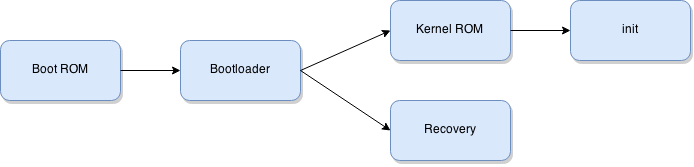
\includegraphics[scale=0.4]{images/boot-sequence.png}
      \end{figure}
      
      \item ¿Por qué esta bloqueado si Android es \textit{open source}?.
      
      \item Desbloquearlo implíca perder la garantía del dispositivo $\rightarrow$ impuesto por \emph{Digital Rights Management}.
  \end{itemize}
\end{frame}

\begin{frame}
  \frametitle{Bootloader - Fastboot}
  \begin{itemize}
      \item Protocolo USB.
      
      \item Permite bootear customs ROMs.
      
      \item Permite flashear una partición.     
      
      \item Permite desbloquear el bootloader (solo si el dispositivo lo soporta).      
  \end{itemize}
\end{frame}

\begin{frame}
  \frametitle{Bootloader - Tipos}
  \begin{itemize}
      \item Open bootloader $\rightarrow$ las compañias no lo desean.
      
      \item Locked bootloader $\rightarrow$ \textit{Carrier ID}.
      
      \item Conditionally open bootloader $\rightarrow$ pérdida de garantía.      
  \end{itemize}
\end{frame}

\subsection{Boot.img \& initramfs}
\begin{frame}
  \frametitle{Boot.img \& initramfs - Boot.img}
  \begin{itemize}
      \item Obtención:
      \begin{itemize}      
	  \item Extracción de una imagen original.
	  
	  \item Descarga desde un sitio confiable (CyanogenMod).
      \end{itemize}      
      
      \item División:
      \begin{itemize}
	  \item A través de \textit{unmkbootimg}.
      
	  \item Estructura:
	  \begin{figure}
	    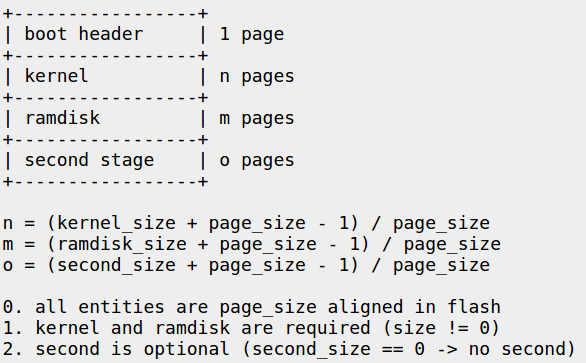
\includegraphics[scale=0.3]{images/boot-image-structure.png}
	  \end{figure}
      \end{itemize}
  \end{itemize}
\end{frame}

\begin{frame}[fragile]
  \frametitle{Boot.img \& initramfs - Initramfs}
  \begin{itemize}
      \item Desempaquetado y descompreción de initramfs:
      \begin{itemize}
	  \item Archivo empaquetado con \textbf{cpio} y comprimido con \textbf{gzip}.
	  
	  \item Archivo \textit{default.prop} $\rightarrow$ contiene propiedades de configuración para la inicialización del sistema.
      \end{itemize}

      \item Habilitar modo inseguro:
      \begin{itemize}
	  \item Propiedad \textit{ro.secure} debe estar en falso $\rightarrow$ demonio de adb (\textit{adbd}) con permisos de \textit{root}.
      \end{itemize}
      
      \item Empaquetar y comprimir initramfs inseguro:
      \begin{itemize}
	  \item A través de \textbf{cpio} y \textbf{gzip} respectivamente.
      \end{itemize}
  \end{itemize}
\end{frame}

\begin{frame}[fragile]
  \frametitle{Boot.img \& initramfs - Reconstrucción de boot.img}
  \begin{itemize}
      \item A través de \textit{mkbootimg}.
      
      \begin{lstlisting}
mkbootimg --kernel zImage --ramdisk insecure_initramfs.cpio.gz --base 0x80200000 --cmdline 'androidboot.hardware=qcom user_debug=31 zcache' -o new_boot.img
      \end{lstlisting}
  \end{itemize}
\end{frame}

\subsection{Booteo/flasheo y testeo}
\begin{frame}[fragile]
  \frametitle{Booteo/flasheo y testeo}
  \begin{itemize}
      \item Booteo (método volátil):
      \begin{lstlisting}
$ fastboot boot new_boot.img
      \end{lstlisting}
      
      \item Flasheo (método no volátil):
      \begin{lstlisting}
$ fastboot flash boot new_boot.img
      \end{lstlisting}
      
      \item Acceso al dispositivo mediante \textit{adb} como usuario \textit{root} en lugar de shell.
      \begin{lstlisting}
$ adb shell
      \end{lstlisting}      
  \end{itemize}
\end{frame}
